\documentclass[runningheads]{llncs}

\usepackage{graphicx}
\usepackage{booktabs}
\usepackage{amsmath,amssymb}
\usepackage{hyperref}
\usepackage{cite}
\usepackage{microtype}
\usepackage{array}
\usepackage{multirow}

\begin{document}

\title{Multi-Temporal Sentinel-2 Spectral-Temporal Features for Seven-Class Crop Classification in Telangana: Spatial Cross-Validation and Independent Test Evaluation\thanks{Working Title for Framework Context: \emph{AI-Based Remote Sensing Framework for Crop Monitoring and Irrigation Decision Support Using Multi-Temporal Sentinel-2 Satellite Imagery}}}

\titlerunning{Multi-Temporal Sentinel-2 Seven-Class Crop Classification in Telangana}

% Anonymized for Double-Blind Review
\author{Anonymous Authors for Double-Blind Peer Review}
\authorrunning{Anonymous et al.}
\institute{Paper submitted to ICIDA 2026 for Double-Blind Review\\
\email{author-email-placeholder@conference.org}}

\maketitle

\begin{abstract}
Accurate, parcel-level crop-type classification in smallholder agricultural landscapes is fundamental for regional food security, yield forecasting, and future agricultural water management. However, in semi-arid tropical regions such as Telangana, India, smallholder agricultural mapping is severely challenged by parcel fragmentation (median area $\sim 0.28$\,ha), optical cloud contamination during the monsoon season, extreme class imbalance, and performance over-optimism induced by spatial autocorrelation under conventional random train/test splits. In this study, we present an end-to-end, reproducible remote sensing and machine learning methodology that classifies seven major agricultural crops (\textbf{Paddy, Cotton, Maize, Bengal Gram, Groundnut, Chillies, and Red Gram}) using multi-temporal Sentinel-2 surface reflectance imagery. We engineer a 140-dimensional Spectral-Temporal ($S+T$) feature space combining full-season aggregations, phenological window compositing across early-season vegetative establishment, mid-season reproductive peak, and late-season senescence, alongside four dynamic transition trajectory deltas. To ensure authentic validation, we enforce strict 5-fold spatial cross-validation grouped by Sub-District (116 Mandals, zero Mandal group overlap) on $N = 7{,}843$ validated farm parcels, coupled with fold-internal inverse-frequency sample weighting. Our primary regularized XGBoost model achieves a pooled out-of-fold Macro-F1 score of \textbf{0.7226}, Balanced Accuracy of \textbf{0.7180}, and Overall Accuracy of \textbf{0.7881 (78.81\%)} across cross-validation. Fold-internal weighting rescues minority Red Gram F1-score from 0.3683 to 0.4420 (+7.37 percentage points). Furthermore, incorporating 20 Gray-Level Co-occurrence Matrix (GLCM) spatial texture features provided no statistically supported global improvement ($p = 0.8600$, 95\% CI $[-0.0066, +0.0092]$), while parcel-area stratification revealed a performance reduction on the smallest parcel quartile ($<1{,}257\,\text{m}^2$, $\Delta = -0.0133$), consistent with the physical hypothesis of boundary pixel contamination. We further evaluate the frozen champion model on an independent intra-state administrative holdout of $N = 2{,}718$ surveyed farm parcels spanning 35 unseen Mandals within Telangana (zero Mandal overlap with training). Across the $N = 2{,}265$ parcels (83.33\% of the surveyed cohort) where satellite features were successfully extracted across all four temporal windows, the frozen model achieves a Macro-F1 of \textbf{0.7308}, Balanced Accuracy of \textbf{0.7326}, and Overall Accuracy of \textbf{0.8155 (81.55\%)}, with 1,847 correct and 418 incorrect predictions. We document that persistent cloud cover caused the exclusion of 453 test parcels (16.67\%), with exclusion rates varying from 4.17\% on dry-season pulses to 25.91\% on monsoon paddy. The metric parity between cross-validation and independent test evaluation confirms the stability of the 140-feature representation across unseen administrative units within the state, while highlighting the necessity of accounting for cloud-driven attrition in operational agricultural monitoring.

\keywords{Crop Classification \and Sentinel-2 \and Multi-Temporal Remote Sensing \and Spatial Cross-Validation \and Smallholder Agriculture \and XGBoost \and Class Imbalance \and Telangana.}
\end{abstract}

\section{Introduction}
Accurate, timely, and spatially explicit crop-type maps are essential for agricultural monitoring, subsidy allocation, agricultural insurance verification, and regional water resource stewardship \cite{defourny2019,griffiths2019}. In semi-arid agrarian economies such as the state of Telangana in southern India, crop production is highly dynamic, relying on a complex mosaic of rainfed cultivation, minor tank storage, and expanding lift-irrigation networks \cite{gumma2020}. Farmers cultivate a diverse portfolio of summer and winter crops across distinct seasons (\emph{Kharif} and \emph{Rabi}), including major cereals (Paddy, Maize), industrial fibers (Cotton), high-value spices (Chillies), and protein-rich pulses and oilseeds (Groundnut, Bengal Gram, Red Gram). However, conventional agricultural statistics in the region rely heavily on manual field-by-field revenue inspections (\emph{patwari} surveys), which are labor-intensive, logistically demanding, prone to reporting latency, and aggregated to coarse administrative levels.

Satellite remote sensing provides an objective, scalable alternative for parcel-level crop mapping. The European Space Agency's (ESA) Copernicus Sentinel-2 constellation offers multispectral imagery at 10\,m and 20\,m spatial resolutions with a 5-day nominal revisit frequency, establishing an unprecedented capability for agricultural monitoring \cite{defourny2019,inglada2015}. Nevertheless, operational crop classification in smallholder environments faces four major scientific and practical hurdles:
\begin{enumerate}
    \item \textbf{Spectral Ambiguity in Fragmented Landscapes:} Smallholder agricultural holdings in Telangana are intensely fragmented, with a median parcel area of approximately 0.28\,ha ($2{,}779\,\text{m}^2$). At this scale, individual farm plots span only a few 10-meter pixels. Multiple co-occurring crops exhibit near-identical spectral reflectance during peak vegetative growth, making single-date optical acquisitions insufficient for reliable discrimination \cite{jin2019,vuolo2018}.
    \item \textbf{Spatial Autocorrelation and Evaluation Bias:} A critical flaw in much of the applied remote-sensing machine learning literature is the reliance on naive random $k$-fold cross-validation or unstratified random train/test splits \cite{meyer2018,roberts2017}. Because neighboring farm fields share identical soil types, micro-climates, irrigation canal access, and planting dates, spatial autocorrelation induces severe data leakage between training and evaluation subsets \cite{roberts2017}.
    \item \textbf{Severe Class Imbalance and Minority Erasure:} Agrarian land use is heavily skewed toward dominant cash crops such as Paddy and Cotton. High-value or subsistence pulses, such as Red Gram (\emph{Cajanus cajan}), frequently represent less than 3\% of regional farm parcels \cite{maxwell2018}.
    \item \textbf{Cloud-Driven Data Missingness:} The \emph{Kharif} cropping cycle coincides with the Southwest monsoon, generating dense, persistent cloud and cloud-shadow cover across optical acquisitions, resulting in parcel-level extraction failures.
\end{enumerate}

\subsection{Scope Demarcation}
To maintain strict scientific integrity, we explicitly define the implemented scope of this study. While the broader conceptual framework envisions an integrated pipeline coupling crop identification with disease diagnosis, crop water stress retrieval, and FAO-56 Penman-Monteith irrigation decision support, \textbf{the experimentally evaluated and validated contribution of this paper is seven-class crop-type classification}. Downstream secondary tasks represent planned future extensions and are not presented as validated operational systems.

\subsection{Primary Contributions}
\begin{enumerate}
    \item \textbf{Multi-Temporal Phenological Feature Engineering:} We design a 140-dimensional Spectral-Temporal ($S+T$) feature space combining full-season statistics, three phenological window aggregations, and four transition trajectory deltas, demonstrating an +8.95 percentage point Macro-F1 gain over the static full-season baseline ($0.6174 \to 0.7069$) from multi-temporal windowing, rising to 0.7226 (+10.52 pp total) with fold-internal class weighting.
    \item \textbf{Strict Spatial Group Cross-Validation:} We enforce 5-fold \texttt{StratifiedGroupKFold} validation partitioned strictly by Sub-District (116 Mandals, zero Mandal overlap), proving that regularized XGBoost achieves a robust pooled Macro-F1 of 0.7226 and Overall Accuracy of 78.81\% across 7,843 parcels without village co-location leakage.
    \item \textbf{Evaluation of Spatial Texture in Smallholder Parcels:} We demonstrate that incorporating 20 GLCM spatial texture features yields no statistically supported overall gain ($p = 0.8600$, 95\% CI $[-0.0066, +0.0092]$) and is associated with reduced performance in the smallest parcel quartile ($<1{,}257\,\text{m}^2$, $\Delta = -0.0133$), providing an empirical basis for selecting the parsimonious 140-feature representation.
    \item \textbf{Leak-Free Minority Pulse Recovery:} We implement fold-internal inverse-frequency sample weighting, boosting Red Gram F1-score from 0.3683 to 0.4420 (+7.37 pp) while preserving strict spatial validation boundaries.
    \item \textbf{Independent Intra-State Administrative Holdout with Cloud Accounting:} We execute frozen-model inference on an independent intra-state administrative holdout of 2,718 surveyed parcels across 35 unseen Mandals in Telangana (zero Mandal overlap with training), establishing that the model achieves 0.7308 Macro-F1 and 81.55\% accuracy on the 2,265 successfully extracted parcels while transparently documenting a 16.67\% cloud-exclusion rate.
\end{enumerate}

\section{Related Work}
\subsection{Multi-Temporal Satellite Optical Mapping}
Early automated crop mapping relied heavily on Landsat or MODIS imagery \cite{inglada2015,gumma2022}. The advent of Sentinel-2 MSI transformed smallholder mapping by providing 10-meter visible and near-infrared bands alongside red-edge spectral bands \cite{defourny2019}. Vuolo et al. \cite{vuolo2018} demonstrated that multi-temporal Sentinel-2 acquisitions increased classification accuracy by 5\% to 17\% compared to single-date imagery. Similarly, Griffiths et al. \cite{griffiths2019} proved that intra-annual phenological compositing metrics effectively separate spectrally overlapping crops. In India, Gumma et al. \cite{gumma2020} demonstrated the utility of Sentinel-2 NDVI time series for mapping field-level pulse and cereal crops in semi-arid environments, while Gumma et al. \cite{gumma2022} established cloud-based machine learning workflows on Google Earth Engine for multi-cropland products across South Asia.

\subsection{Spatial Cross-Validation and Spatial Autocorrelation}
The necessity of spatial blocking in geospatial machine learning has been established by Roberts et al. \cite{roberts2017} and Meyer et al. \cite{meyer2018}. Spatial autocorrelation violates the fundamental assumption that training and validation instances are independently and identically distributed. Roberts et al. \cite{roberts2017} documented that non-spatial cross-validation can underestimate true prediction error by 20\% to 60\% in spatially structured datasets.

\subsection{Class Imbalance and Cost-Sensitive Learning}
As noted by Maxwell et al. \cite{maxwell2018}, standard loss functions in gradient-boosted decision trees optimize global error rates at the expense of minority classes. Inverse-frequency sample weighting adjusts the gradient contribution of each class according to its empirical rarity, providing a principled mechanism to recover minority decision boundaries without distorting physical feature distributions \cite{chen2016,maxwell2018}.

\subsection{Smallholder Parcel Fragmentation and Spatial Texture}
In smallholder systems, individual field extents are often smaller than 0.5\,ha \cite{jin2019}. While spatial texture metrics, such as Haralick's Gray-Level Co-occurrence Matrix (GLCM; \cite{haralick1973}), have demonstrated value in homogeneous commercial farms \cite{vuolo2018}, Lebourgeois et al. \cite{lebourgeois2017} highlighted that plots under 0.25\,ha suffer from severe boundary contamination.

\section{Study Area and Dataset}
\subsection{Study Area}
The study was conducted across the state of Telangana in southern India (Fig.~\ref{fig:spatial_overview}), covering an area of approximately $112{,}077\,\text{km}^2$. The region experiences a semi-arid tropical climate characterized by three distinct seasons: the Southwest monsoon (\emph{Kharif}, June to October), the dry winter (\emph{Rabi}, November to March), and a hot summer (March to May). Annual rainfall ranges between 700\,mm and 1,200\,mm.

\begin{figure}[t]
\centering
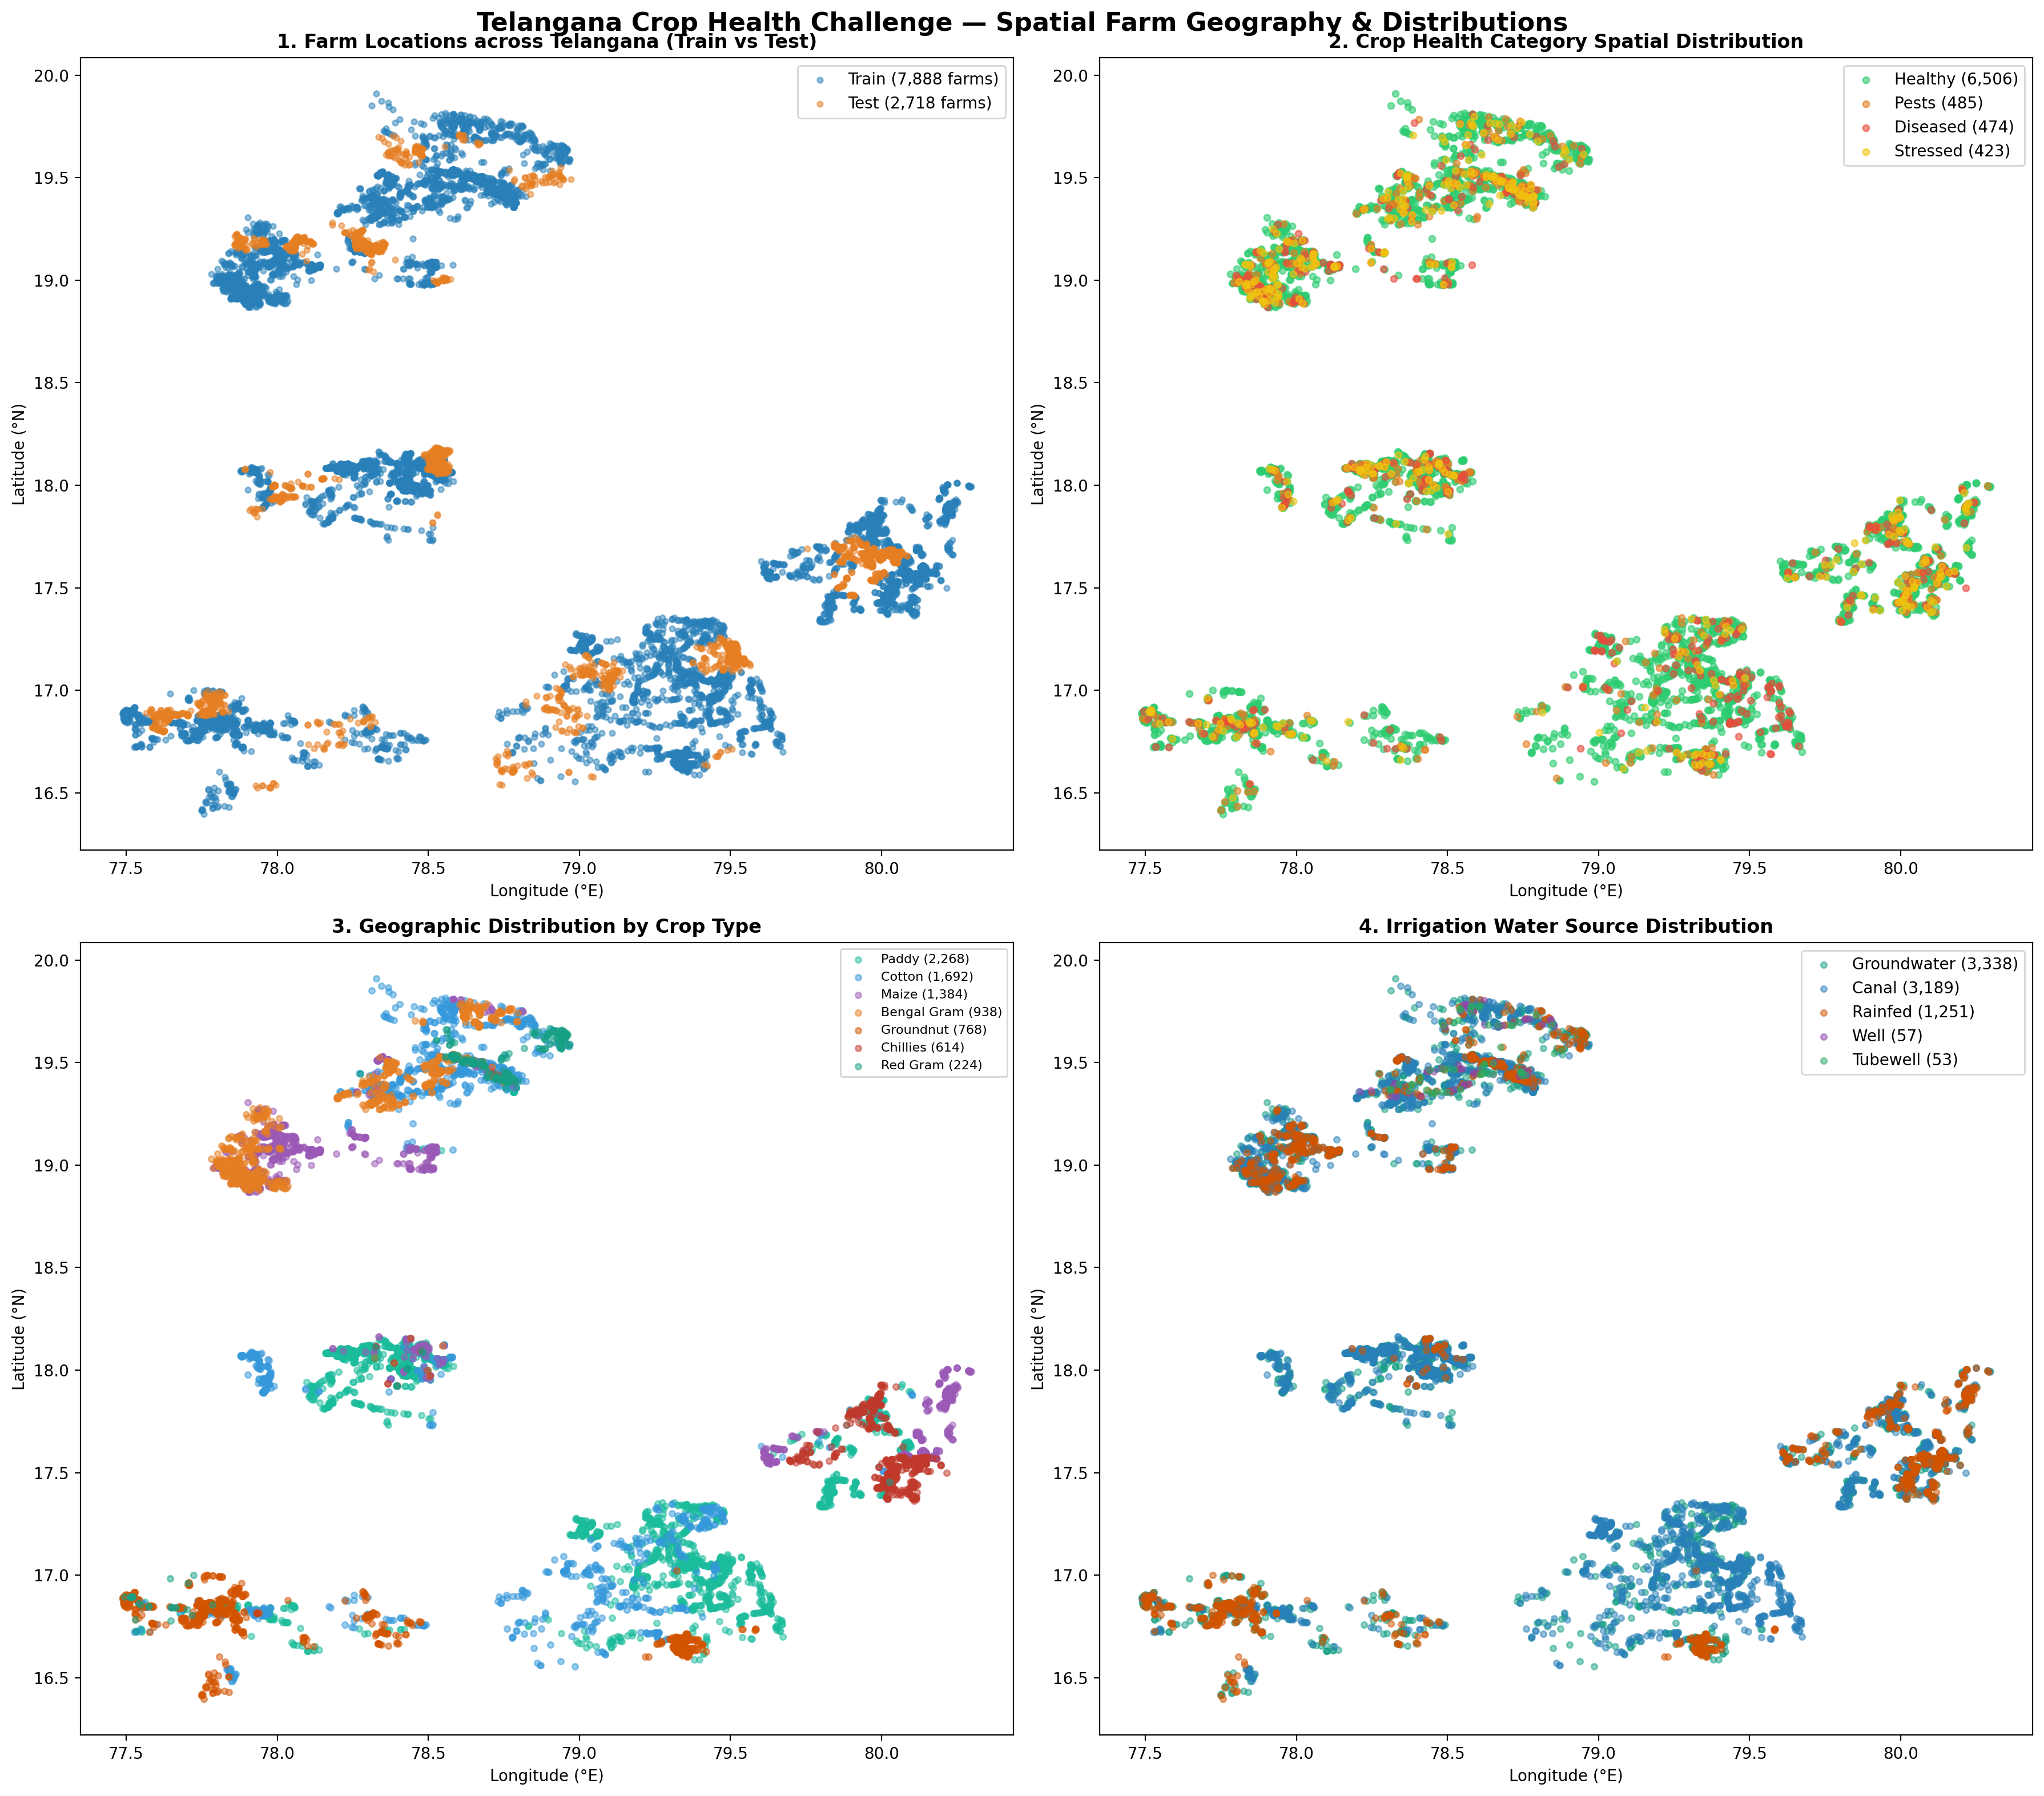
\includegraphics[width=0.75\textwidth]{outputs/figures/telangana_spatial_overview.png}
\caption{Spatial distribution of training (116 Mandals) and independent test (35 Mandals) agricultural parcels across Telangana, India.}
\label{fig:spatial_overview}
\end{figure}

\subsection{Ground-Truth Parcel Cohorts}
The empirical ground-truth dataset consists of verified vector polygons derived from extensive field surveys conducted across Telangana:
\begin{enumerate}
    \item \textbf{Training Cohort (\texttt{Train.csv}):} 7,888 initial surveyed parcel polygons across 14 districts and 116 Mandals, yielding an authoritative cohort of $N = 7{,}843$ eligible farm parcels following topological and cloud validation.
    \item \textbf{Independent Test Cohort (\texttt{Test.csv}):} $N = 2{,}718$ farm parcels distributed across 35 Mandals in 12 districts within Telangana. A preflight spatial audit confirmed zero Mandal overlap with training, establishing an independent intra-state administrative holdout across unseen Mandals within Telangana (Table~\ref{tab:cohort}). Ten broader districts overlap between cohorts; disjoint Mandals provide administrative separation but do not guarantee geographic independence or zero spatial autocorrelation.
    \item \textbf{Target Nomenclature:} Seven crop classes: \textbf{Bengal Gram, Chillies, Cotton, Groundnut, Maize, Paddy, and Red Gram}.
\end{enumerate}

\begin{table}[t]
\centering
\caption{Cohort Composition and Spatial Partitioning.}
\label{tab:cohort}
\small
\begin{tabular}{lcc}
\toprule
\textbf{Cohort Property} & \textbf{Training Cohort} & \textbf{Independent Test Cohort} \\
\midrule
Initial Surveyed Parcels & 7,888 & 2,718 \\
Persistent Cloud / Shadow Failures & 45 (0.57\%) & 453 (16.67\%) \\
Eligible Evaluated Parcels & \textbf{7,843 (99.43\%)} & \textbf{2,265 (83.33\%)} \\
Administrative Units (Mandals) & 116 & 35 \\
Districts Covered & 14 & 12 (10 districts overlap) \\
Inter-Cohort Mandal Overlap & — & \textbf{0 Mandals (Disjoint Holdout)} \\
Validation Design & 5-Fold \texttt{StratifiedGroupKFold} & Frozen Out-of-Mandal Inference \\
Target Variable & \texttt{Crop} (7 Classes) & \texttt{Crop} (7 Classes) \\
\bottomrule
\end{tabular}
\end{table}

\begin{table}[t]
\centering
\caption{Parcel-Level Feature Extraction Coverage \& Cloud Exclusion Accounting.}
\label{tab:cloud}
\small
\begin{tabular}{lccccc}
\toprule
\textbf{Crop Class} & \textbf{Total Test} & \textbf{Evaluated} & \textbf{Excluded} & \textbf{Coverage (\%)} & \textbf{Loss (\%)} \\
\midrule
Bengal Gram & 48 & 46 & 2 & 95.83\% & 4.17\% \\
Groundnut & 266 & 241 & 25 & 90.60\% & 9.40\% \\
Maize & 699 & 631 & 68 & 90.27\% & 9.73\% \\
Red Gram & 41 & 35 & 6 & 85.37\% & 14.63\% \\
Cotton & 569 & 472 & 97 & 82.95\% & 17.05\% \\
Chillies & 381 & 311 & 70 & 81.63\% & 18.37\% \\
Paddy & 714 & 529 & 185 & 74.09\% & \textbf{25.91\%} \\
\midrule
\textbf{Total Cohort} & \textbf{2,718} & \textbf{2,265} & \textbf{453} & \textbf{83.33\%} & \textbf{16.67\%} \\
\bottomrule
\end{tabular}
\end{table}

\section{Proposed Methodology}
\subsection{Satellite Preprocessing and Cloud Masking}
Multi-temporal surface reflectance imagery was ingested from Copernicus Sentinel-2 Level-2A (\texttt{COPERNICUS/S2\_SR\_HARMONIZED}) via Google Earth Engine (GEE). Non-vegetated and compromised pixels were identified and masked using the Scene Classification Layer (SCL).

\subsection{Phenological Windowing and Feature Representation}
We establish four temporal extraction windows tailored to Telangana's calendar: Early Season (Jun 01--Jul 31), Mid Season (Aug 01--Sep 30), Late Season (Oct 01--Nov 30), and Full Season (Jun 01--Dec 31). Ten surface reflectance bands (B2, B3, B4, B5, B6, B7, B8, B8A, B11, B12) and 14 vegetation/water indices (NDVI, EVI, NDMI, NDWI, GNDVI, NDRE, MSAVI, CI$_\text{Green}$, CI$_\text{RedEdge}$, MSI, NDBI, SAVI, SIPI, NMDI) were extracted per window (34 features $\times 4 = 136$). Adding four phenological transition deltas ($\Delta_\text{growth}$, $\text{Ratio}_\text{peak/early}$, $\Delta_\text{senescence}$, $\Delta_\text{moisture}$) yields the exact \textbf{140-dimensional Spectral-Temporal ($S+T$) feature space} (Table~\ref{tab:features}).

\begin{table}[t]
\centering
\caption{140-Dimensional Spectral-Temporal Feature Representation.}
\label{tab:features}
\small
\begin{tabular}{lllcc}
\toprule
\textbf{Feature Group} & \textbf{Temporal Window} & \textbf{Description} & \textbf{Count} \\
\midrule
Spectral \& Biophysical ($S$) & Full Season (Jun 01--Dec 31) & 10 S2 bands + 14 spectral indices & 34 \\
Windowed Phenology ($W_1$) & Early Season (Jun 01--Jul 31) & Emergence / establishment & 34 \\
Windowed Phenology ($W_2$) & Mid Season (Aug 01--Sep 30) & Peak vegetative vigor / flowering & 34 \\
Windowed Phenology ($W_3$) & Late Season (Oct 01--Nov 30) & Maturation / senescence & 34 \\
Dynamic Deltas ($T$) & Multi-Window Trajectories & $\Delta_\text{growth}$, $\text{Ratio}$, $\Delta_\text{senesc}$, $\Delta_\text{moist}$ & 4 \\
\midrule
\textbf{Total Dimensionality} & — & \textbf{Spectral-Temporal Vector ($S+T$)} & \textbf{140} \\
\bottomrule
\end{tabular}
\end{table}

\subsection{Spatial Texture Features}
We constructed an augmented 160-dimensional representation ($S+T+P$) by extracting Gray-Level Co-occurrence Matrix (GLCM; \cite{haralick1973}) texture rasters across NIR (B8) at 10-meter resolution using a $3\times3$ sliding window (5 statistics $\times 4$ windows = 20 features).

\subsection{Model Architecture and Class Weighting}
We deploy XGBoost \cite{chen2016} with inverse-frequency sample weights $w_c$:
\begin{equation}
w_c = \frac{N_\text{train}}{C \cdot N_c}
\end{equation}
computed strictly inside each training fold to prevent validation leakage.

\subsection{Spatial Validation and Hyperparameter Protocol}
Validation is structured as a 5-fold \texttt{StratifiedGroupKFold} grouped by Mandal. Hyperparameters were evaluated via an exploratory bounded search of ten candidate configurations using 3-fold grouped inner cross-validation strictly on the training partition of Outer Fold 0 ($N = 6{,}335$ parcels across 93 Mandals; Outer Fold 0 validation partition has $N = 1{,}508$ parcels across 23 Mandals). Selection was based on inner Macro-F1 (0.6797). The selected configuration—\texttt{max\_depth=7}, \texttt{learning\_rate=0.05}, \texttt{n\_estimators=300}, \texttt{subsample=0.80}, \texttt{colsample\_bytree=0.75}, \texttt{min\_child\_weight=3}, \texttt{gamma=0.20}, \texttt{reg\_alpha=0.20}, and \texttt{reg\_lambda=5.0}—was frozen and evaluated across all 5 spatial folds and test inference (Table~\ref{tab:hyperparams}). This protocol is an exploratory parameter search on a single fold rather than fully nested cross-validation.

\begin{table}[t]
\centering
\caption{XGBoost Hyperparameter Specification and Tuning Protocol.}
\label{tab:hyperparams}
\small
\begin{tabular}{lccl}
\toprule
\textbf{Hyperparameter} & \textbf{Selected} & \textbf{Search Space} & \textbf{Tuning Protocol \& Context} \\
\midrule
\texttt{n\_estimators} & 300 & [100, 200, 300, 500] & Fixed during exploration \\
\texttt{max\_depth} & 7 & [5, 6, 7, 8] & Captures non-linear canopy interactions \\
\texttt{learning\_rate} ($\eta$) & 0.05 & [0.03, 0.05, 0.10] & Conservative shrinkage \\
\texttt{subsample} & 0.80 & [0.70, 0.80, 0.90] & Row sub-sampling per boosting iteration \\
\texttt{colsample\_bytree} & 0.75 & [0.60, 0.75, 0.80, 1.00] & Feature sub-sampling per tree split \\
\texttt{min\_child\_weight} & 3 & [1, 3, 5] & Prevents fitting smallholder clusters \\
\texttt{gamma} & 0.20 & [0.0, 0.1, 0.2, 0.3] & Minimum loss reduction to split leaf \\
\texttt{reg\_lambda} ($L_2$) & 5.0 & [1.0, 2.0, 3.0, 5.0, 10.0] & L2 regularization against spatial noise \\
\texttt{reg\_alpha} ($L_1$) & 0.20 & [0.0, 0.1, 0.2, 0.5, 1.0] & Mild sparsity enforcement \\
\texttt{tree\_method} & \texttt{hist} & [\texttt{hist}] & Fast exact histogram binning \\
Class Weighting & Inverse-Freq & [None, Bal, Inv-Freq] & $w_c = N / (C \cdot N_c)$; fold-internal \\
\bottomrule
\end{tabular}
\end{table}

\section{Results and Discussion}
\subsection{Spatial Cross-Validation Benchmark}
Across $N = 7{,}843$ parcels in 116 Mandals, the primary \texttt{Weighted S+T} model achieves pooled Macro-F1 of \textbf{0.7226}, Balanced Accuracy of \textbf{0.7180}, and Overall Accuracy of \textbf{0.7881 (78.81\%)} (Table~\ref{tab:cv}). Fold-mean Macro-F1 is $0.7117 \pm 0.0181$ (population SD) or $\pm 0.0202$ (sample SD) (Fig.~\ref{fig:fold_var}).

\begin{table}[t]
\centering
\caption{5-Fold Spatial Cross-Validation Performance (\texttt{Weighted S+T}, $N=7,843$).}
\label{tab:cv}
\small
\begin{tabular}{lcccccc}
\toprule
\textbf{Fold ID} & \textbf{Val Mandals} & \textbf{Val Parcels} & \textbf{Macro-F1} & \textbf{Accuracy} & \textbf{Bal-Acc} & \textbf{W-F1} \\
\midrule
Fold 0 & 23 & 1,508 & 0.7269 & 0.7960 & 0.7203 & 0.7932 \\
Fold 1 & 21 & 1,600 & 0.7381 & 0.8013 & 0.7329 & 0.7997 \\
Fold 2 & 22 & 1,595 & 0.6919 & 0.7717 & 0.6865 & 0.7681 \\
Fold 3 & 26 & 1,530 & 0.6945 & 0.7749 & 0.6911 & 0.7728 \\
Fold 4 & 24 & 1,610 & 0.7073 & 0.7966 & 0.7102 & 0.7946 \\
\midrule
\textbf{Fold Mean} & 23.2 & 1,568.6 & \textbf{0.7117} & \textbf{0.7881} & \textbf{0.7082} & \textbf{0.7857} \\
\textbf{Pooled} & \textbf{116} & \textbf{7,843} & \textbf{0.7226} & \textbf{0.7881} & \textbf{0.7180} & \textbf{0.7857} \\
\bottomrule
\end{tabular}
\end{table}

\begin{figure}[t]
\centering
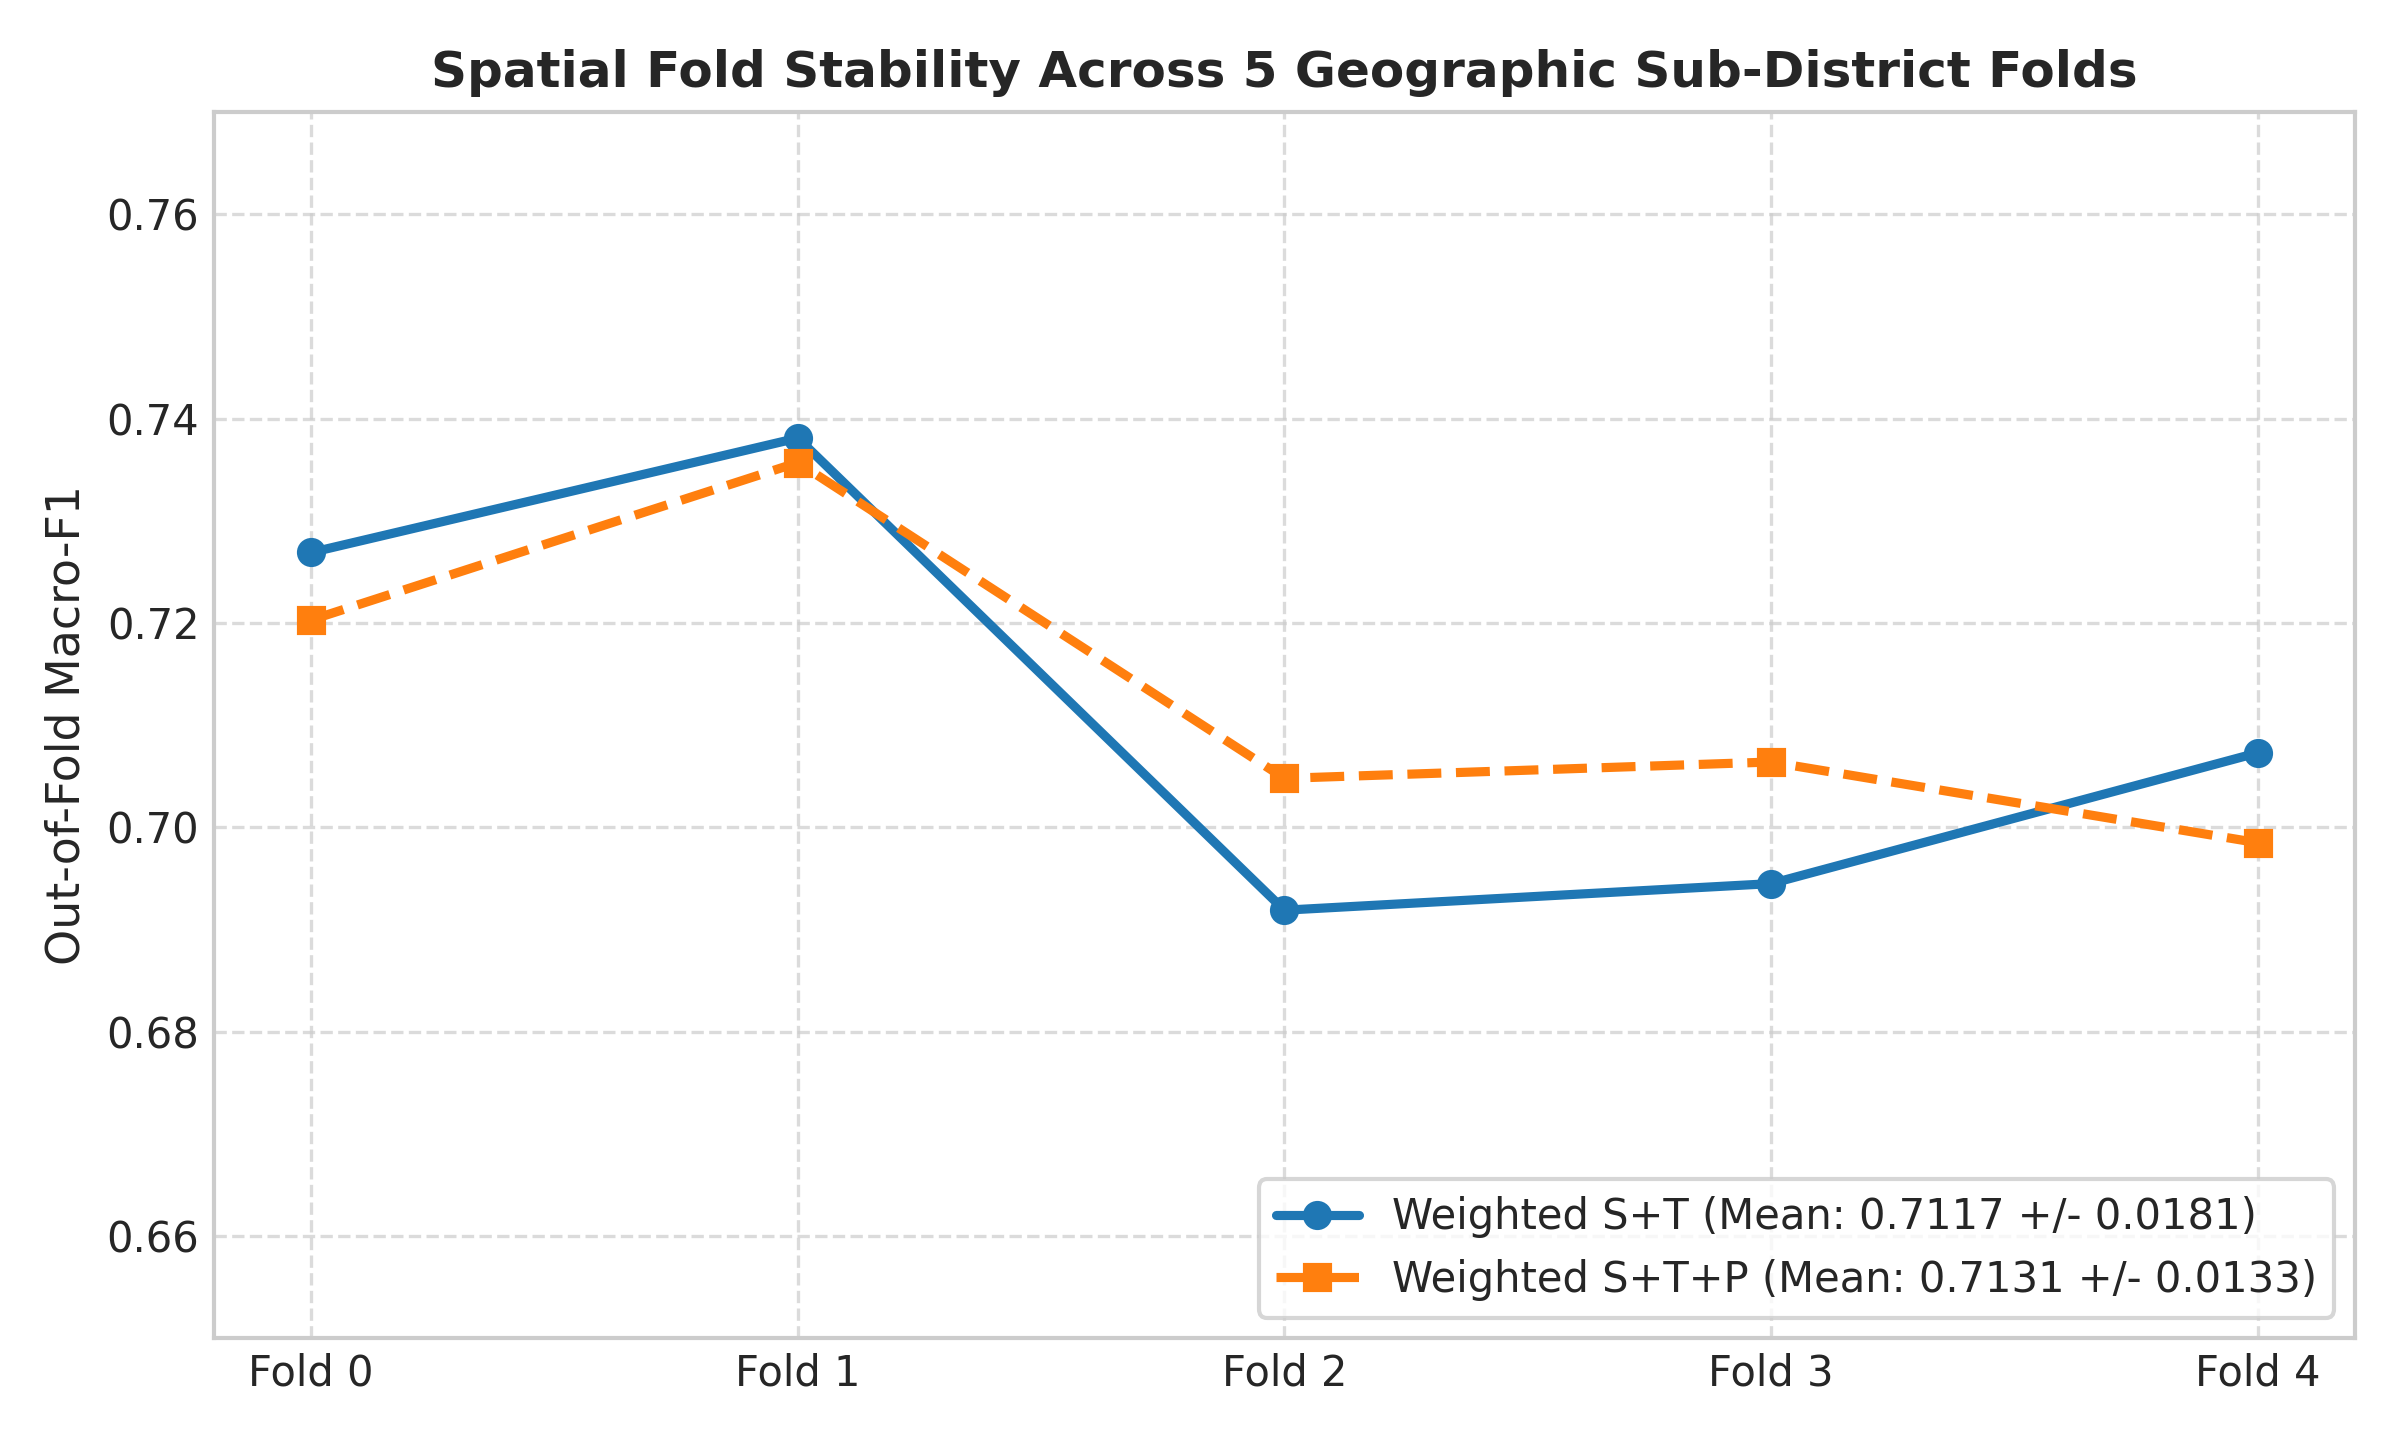
\includegraphics[width=0.7\textwidth]{outputs/reports/paper_materials/figures/fig3_fold_variability.png}
\caption{Performance metric dispersion across 5 outer spatial cross-validation folds.}
\label{fig:fold_var}
\end{figure}

\subsection{Feature Ablation and Systematic Evolution}
Multi-temporal windowing (140 S+T, unweighted) propelled Macro-F1 from 0.6174 (static full-season) to 0.7069 (+8.95 pp gain; Table~\ref{tab:ablation}, Fig.~\ref{fig:ablation}). Fold-internal sample weighting further raised Macro-F1 to 0.7226 (+1.57 pp), rescuing Red Gram F1 from 0.3683 to 0.4420 (+7.37 pp).

\begin{table}[t]
\centering
\caption{Model Evolution, Feature Ablations, and Significance Testing.}
\label{tab:ablation}
\small
\begin{tabular}{lccccc}
\toprule
\textbf{Model / Stage} & \textbf{Feats} & \textbf{Cohort} & \textbf{Weighting} & \textbf{Macro-F1} & \textbf{Accuracy} \\
\midrule
Early Single Window & 34 & 7,843 & Unweighted & 0.5058 & 0.6358 \\
Full Single Window & 34 & 7,843 & Unweighted & 0.6174 & 0.7208 \\
Unweighted S+T & 140 & 7,843 & Unweighted & 0.7069 & 0.7924 \\
Unweighted S+T+P & 160 & 7,843 & Unweighted & 0.7038 & 0.7900 \\
\textbf{Final Weighted S+T} & \textbf{140} & \textbf{7,843} & \textbf{Inverse-Freq} & \textbf{0.7226} & \textbf{0.7881} \\
Weighted S+T+P & 160 & 7,843 & Inverse-Freq & 0.7228 & 0.7905 \\
\bottomrule
\end{tabular}
\end{table}

\begin{figure}[t]
\centering
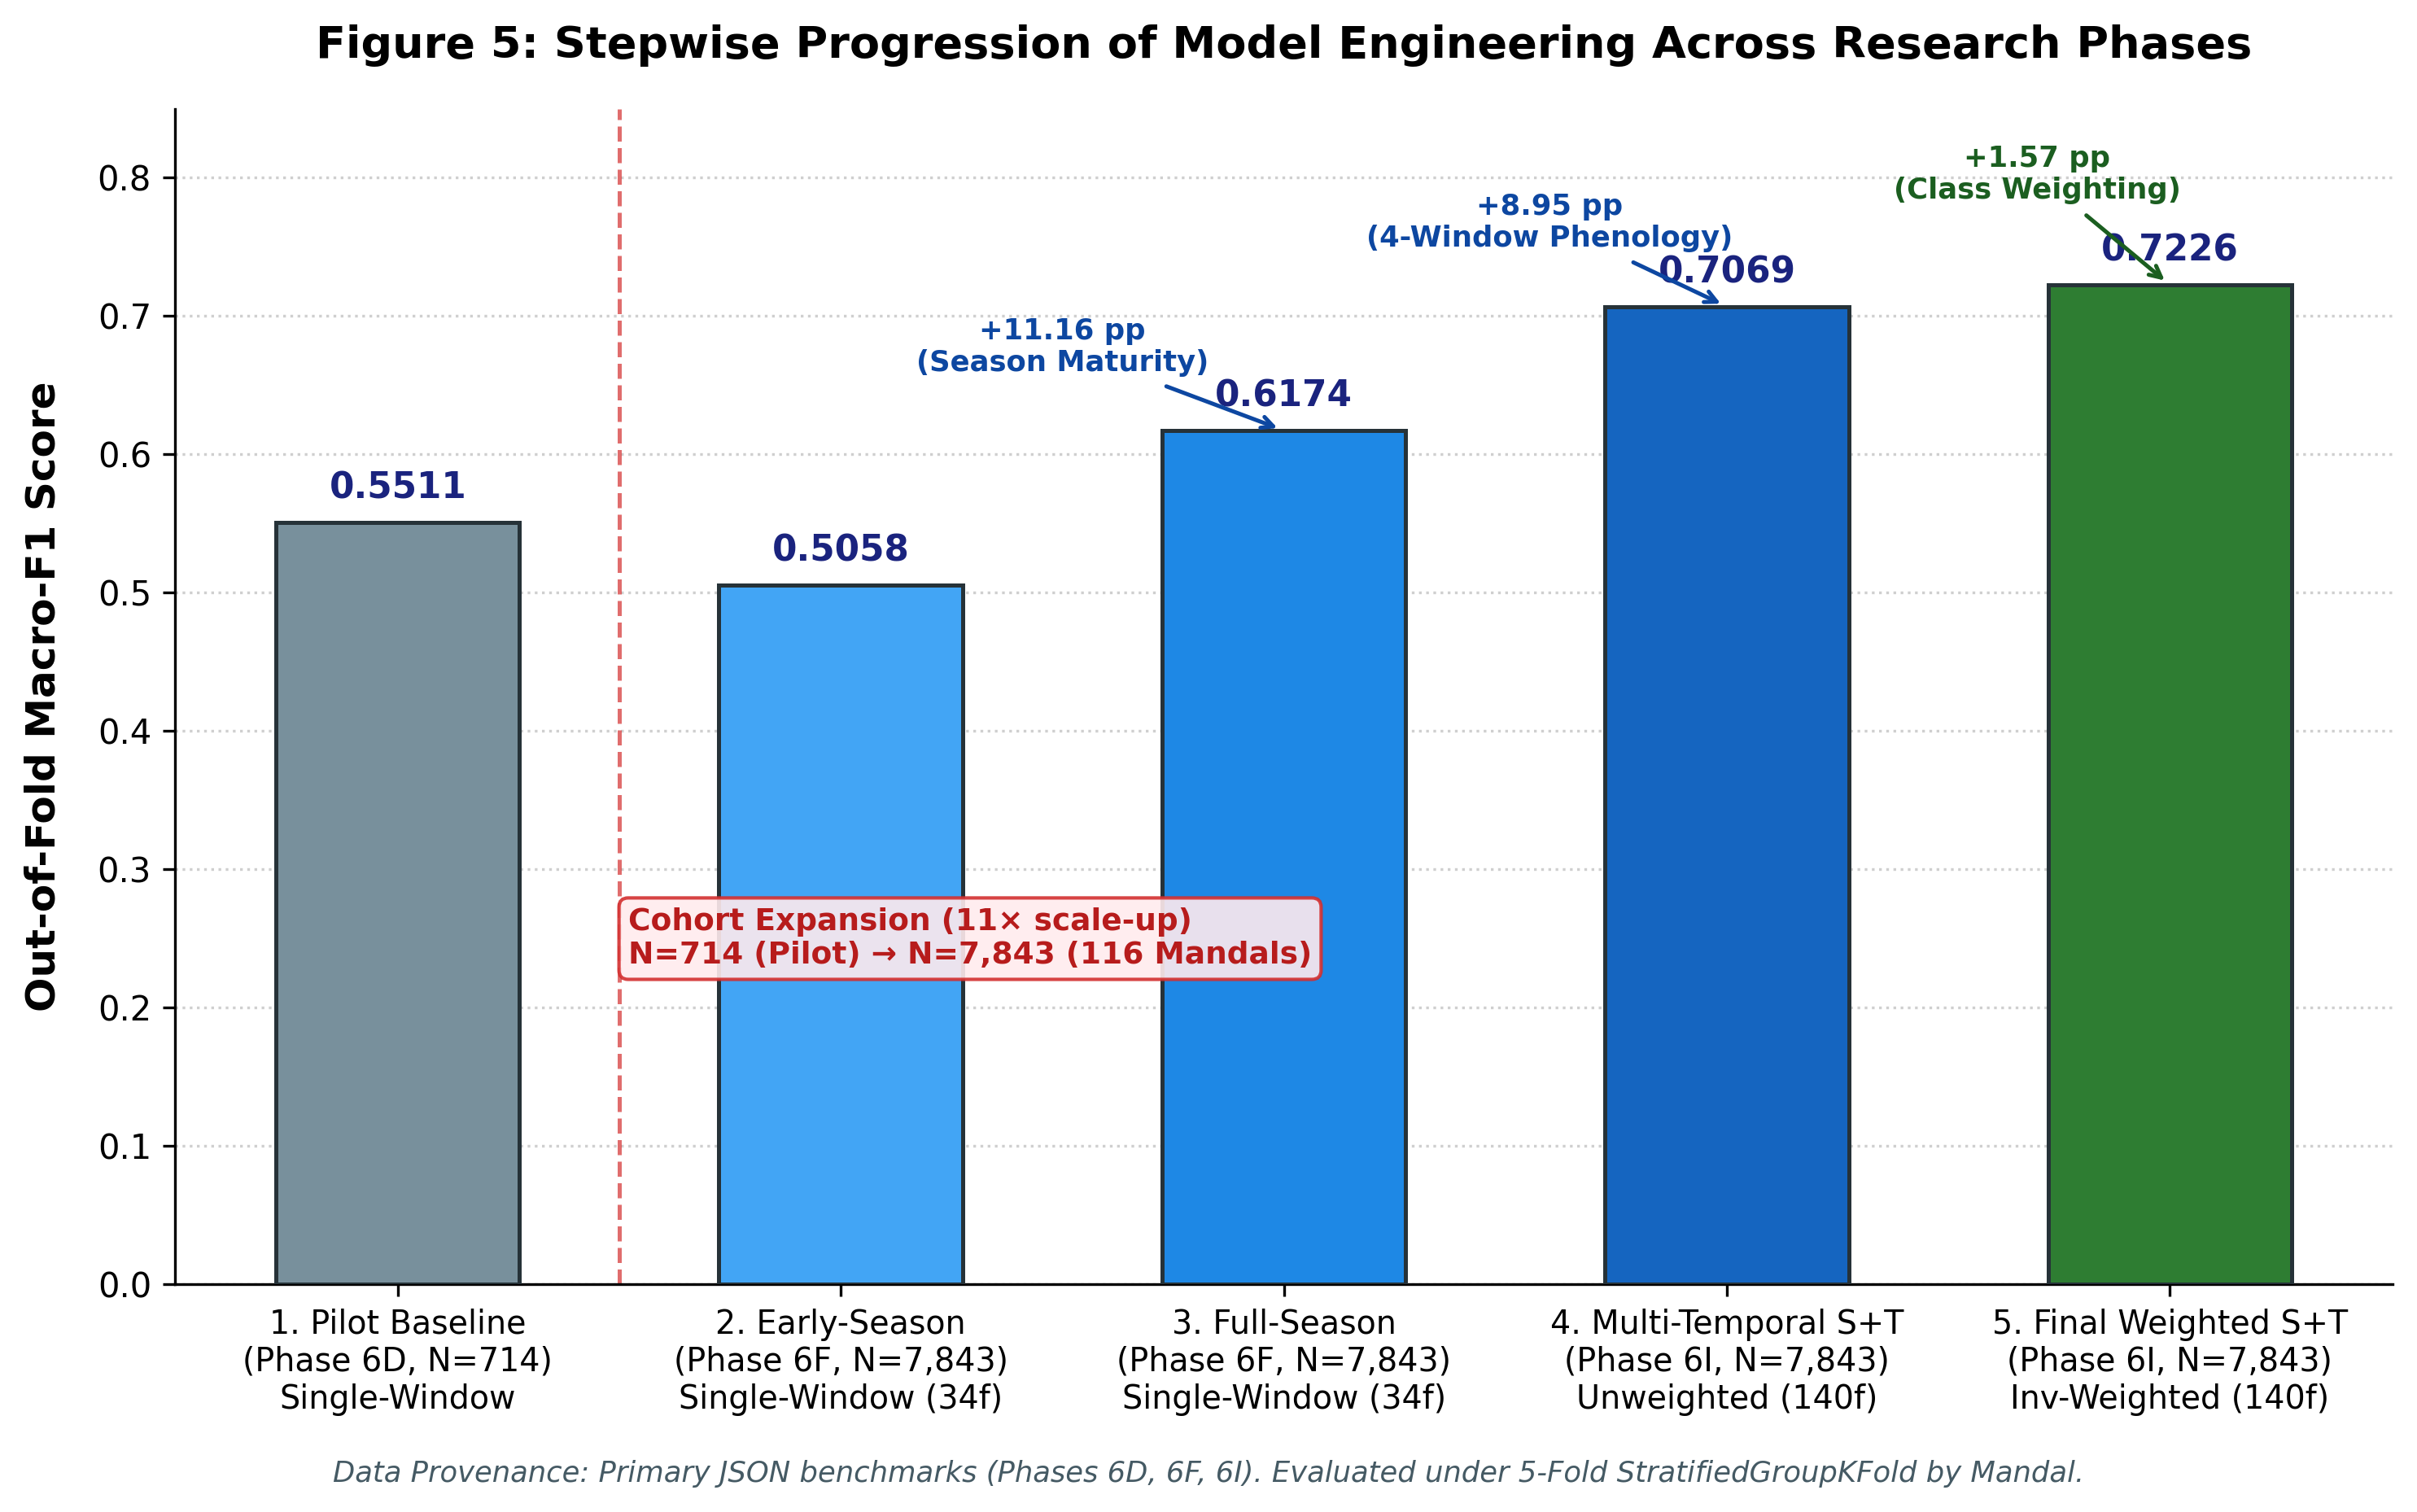
\includegraphics[width=0.7\textwidth]{outputs/reports/paper_materials/figures/fig5_pipeline_evolution.png}
\caption{Stepwise feature ablation progression from single-window baseline to champion weighted S+T pipeline.}
\label{fig:ablation}
\end{figure}

\subsection{Spatial Texture Evaluation and Parcel-Size Stratification}
The 160-dimensional \texttt{Weighted S+T+P} model achieved Macro-F1 of 0.7228, virtually identical to 140-feature \texttt{Weighted S+T} (0.7226, $\Delta = +0.0002$; cluster bootstrap $p = 0.8600$, paired $t$-test $p = 0.7765$). Quartile stratification (Table~\ref{tab:quartiles}, Fig.~\ref{fig:quartiles}) revealed a descriptive drop in Q1 ($<1{,}257\,\text{m}^2$, $\Delta = -0.0133$), consistent with boundary pixel contamination from $3\times3$ ($900\,\text{m}^2$) convolution kernels. Parsimony justifies selecting the 140-feature model.

\begin{table}[t]
\centering
\caption{Parcel Area Quartile Stratification: GLCM Texture vs Spectral-Temporal.}
\label{tab:quartiles}
\small
\begin{tabular}{lccccc}
\toprule
\textbf{Quartile} & \textbf{Area Range ($\text{m}^2$)} & \textbf{Parcels} & \textbf{S+T F1} & \textbf{S+T+P F1} & \textbf{Delta} \\
\midrule
Q1 & 54 – 1,257 & 1,961 & 0.6598 & 0.6465 & -0.0133 (-1.33 pp) \\
Q2 & 1,257 – 2,783 & 1,961 & 0.7332 & 0.7184 & -0.0148 (-1.48 pp) \\
Q3 & 2,784 – 5,517 & 1,960 & 0.7400 & 0.7530 & +0.0130 (+1.30 pp) \\
Q4 & 5,528 – 69,491 & 1,961 & 0.7253 & 0.7219 & -0.0034 (-0.34 pp) \\
\midrule
\textbf{Full} & \textbf{54 – 69,491} & \textbf{7,843} & \textbf{0.7226} & \textbf{0.7228} & \textbf{+0.0002 (+0.02 pp)} \\
\bottomrule
\end{tabular}
\end{table}

\begin{figure}[t]
\centering
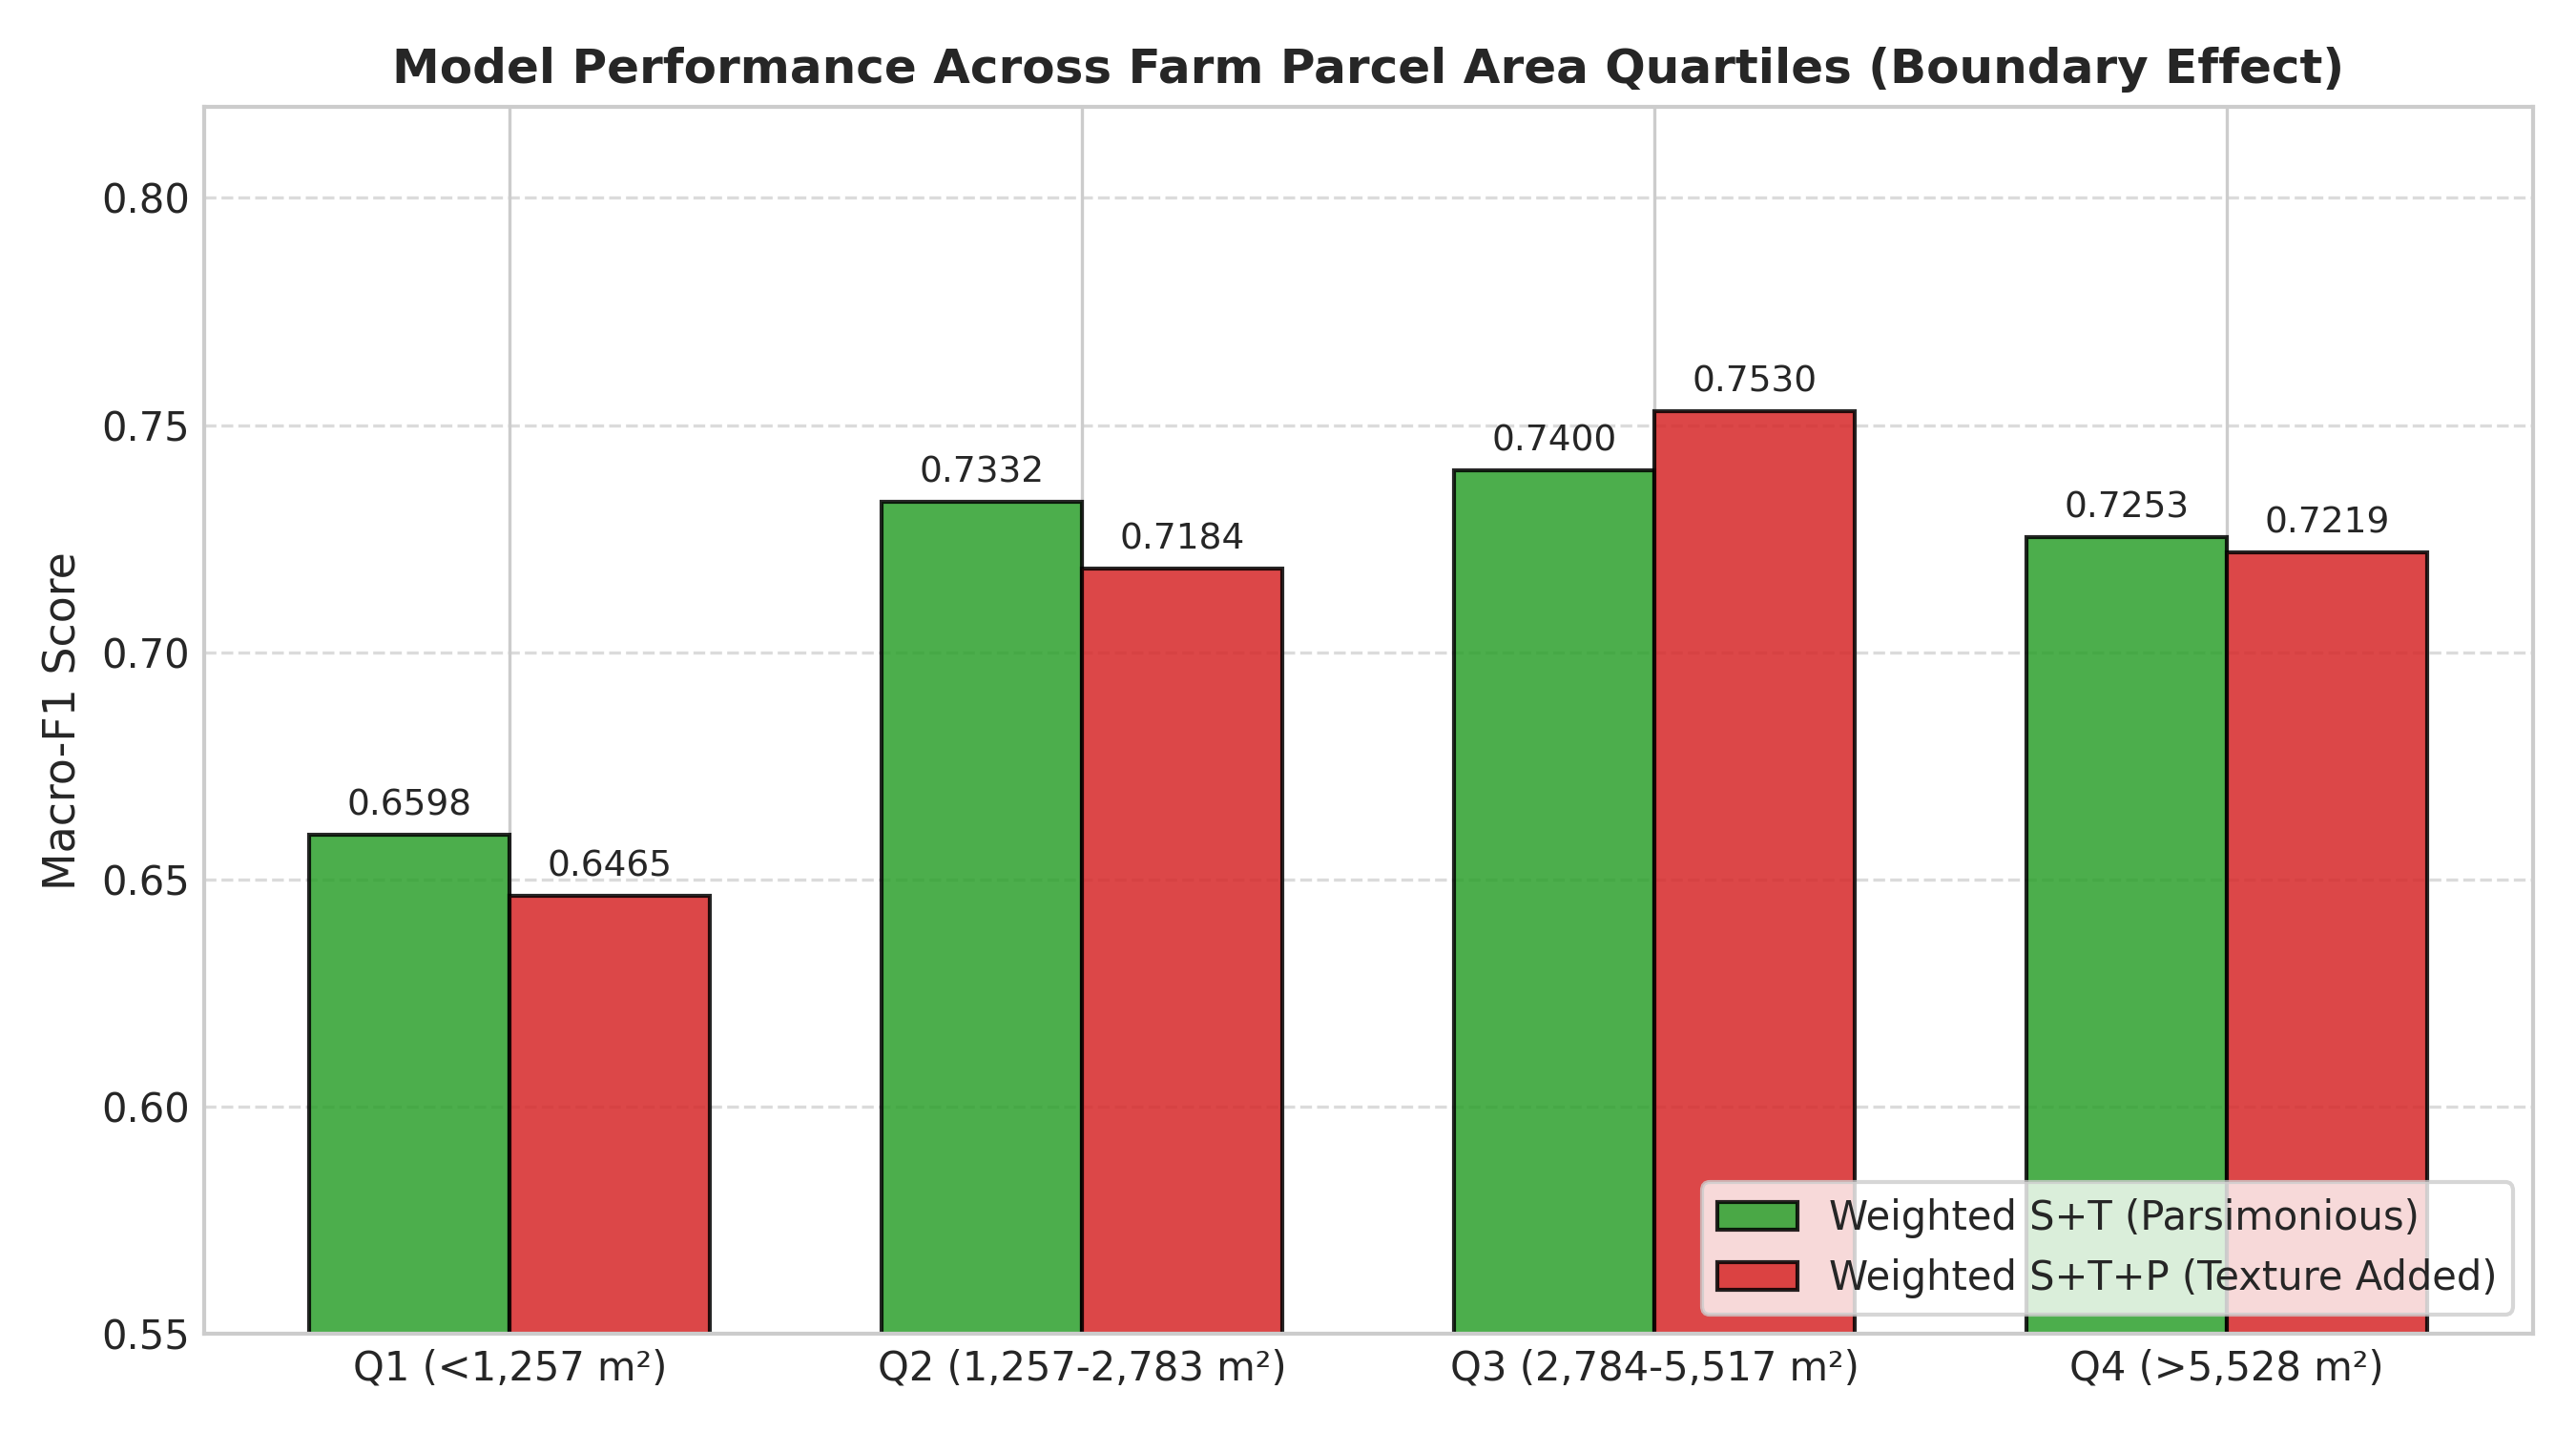
\includegraphics[width=0.7\textwidth]{outputs/reports/paper_materials/figures/fig4_parcel_size_quartiles.png}
\caption{Macro-F1 delta across parcel-area quartiles, illustrating boundary contamination vulnerability in smallholder plots.}
\label{fig:quartiles}
\end{figure}

\subsection{Independent Test Set Evaluation across 35 Unseen Mandals}
On the independent test cohort ($N = 2{,}718$), satellite features were successfully extracted for $N = 2{,}265$ parcels (83.33\%). The frozen model achieved Macro-F1 of \textbf{0.7308}, Overall Accuracy of \textbf{0.8155 (81.55\%)}, Balanced Accuracy of \textbf{0.7326}, and Weighted-F1 of \textbf{0.8137}, with 1,847 correct and 418 incorrect predictions (Table~\ref{tab:test}, Table~\ref{tab:classwise}, Table~\ref{tab:cm}, Fig.~\ref{fig:cm}, Fig.~\ref{fig:classwise}).

\begin{table}[t]
\centering
\caption{Independent Test Performance vs Spatial Cross-Validation Parity.}
\label{tab:test}
\small
\begin{tabular}{lcccc}
\toprule
\textbf{Metric} & \textbf{Spatial CV ($N=7,843$)} & \textbf{Test Set ($N=2,265$)} & \textbf{Delta} \\
\midrule
Macro-F1 & 0.7226 & \textbf{0.7308} & +0.0082 \\
Overall Accuracy & 0.7881 (78.81\%) & \textbf{0.8155 (81.55\%)} & +0.0274 \\
Balanced Accuracy & 0.7180 & \textbf{0.7326} & +0.0146 \\
Weighted-F1 & 0.7857 & \textbf{0.8137} & +0.0280 \\
Evaluated Sample Size & 7,843 & 2,265 & — \\
Excluded Cloud Loss & 45 (0.57\%) & 453 (16.67\%) & — \\
\bottomrule
\end{tabular}
\end{table}

\begin{table}[t]
\centering
\caption{Verified Class-Wise Performance Metrics (Spatial CV vs Independent Test).}
\label{tab:classwise}
\small
\begin{tabular}{lcccccc}
\toprule
\textbf{Crop Class} & \textbf{CV Prec} & \textbf{CV Rec} & \textbf{CV F1} & \textbf{Test Prec} & \textbf{Test Rec} & \textbf{Test F1} \\
\midrule
Bengal Gram & 0.7916 & 0.8667 & 0.8275 & 0.6792 & 0.7826 & 0.7273 \\
Chillies & 0.5249 & 0.5441 & 0.5343 & 0.7409 & 0.7814 & 0.7606 \\
Cotton & 0.7939 & 0.8261 & 0.8097 & 0.7505 & 0.8157 & 0.7817 \\
Groundnut & 0.8597 & 0.8698 & 0.8647 & 0.8340 & 0.8755 & 0.8543 \\
Maize & 0.7492 & 0.6730 & 0.7090 & 0.9016 & 0.7845 & 0.8390 \\
Paddy & 0.8664 & 0.8752 & 0.8708 & 0.8468 & 0.8885 & 0.8672 \\
Red Gram & 0.5467 & 0.3710 & \textbf{0.4420} & 0.5000 & 0.2000 & \textbf{0.2857} \\
\midrule
\textbf{Macro Average} & \textbf{0.7332} & \textbf{0.7180} & \textbf{0.7226} & \textbf{0.7504} & \textbf{0.7326} & \textbf{0.7308} \\
\bottomrule
\end{tabular}
\end{table}

\begin{table}[t]
\centering
\caption{Independent Test Set Confusion Matrix ($N=2,265$).}
\label{tab:cm}
\footnotesize
\begin{tabular}{lcccccccc}
\toprule
\textbf{True $\downarrow$ \textbackslash Pred $\rightarrow$} & \textbf{BG} & \textbf{CH} & \textbf{CO} & \textbf{GN} & \textbf{MZ} & \textbf{PD} & \textbf{RG} & \textbf{Total} \\
\midrule
Bengal Gram (BG) & \textbf{36} & 1 & 4 & 0 & 2 & 1 & 2 & 46 \\
Chillies (CH) & 0 & \textbf{243} & 40 & 5 & 12 & 11 & 0 & 311 \\
Cotton (CO) & 7 & 14 & \textbf{385} & 20 & 15 & 28 & 3 & 472 \\
Groundnut (GN) & 0 & 9 & 11 & \textbf{211} & 6 & 4 & 0 & 241 \\
Maize (MZ) & 6 & 41 & 36 & 12 & \textbf{495} & 40 & 1 & 631 \\
Paddy (PD) & 1 & 18 & 16 & 5 & 18 & \textbf{470} & 1 & 529 \\
Red Gram (RG) & 3 & 2 & 21 & 0 & 1 & 1 & \textbf{7} & 35 \\
\midrule
\textbf{Total Pred} & \textbf{53} & \textbf{328} & \textbf{513} & \textbf{253} & \textbf{549} & \textbf{555} & \textbf{14} & \textbf{2,265} \\
\bottomrule
\end{tabular}
\end{table}

\begin{figure}[t]
\centering
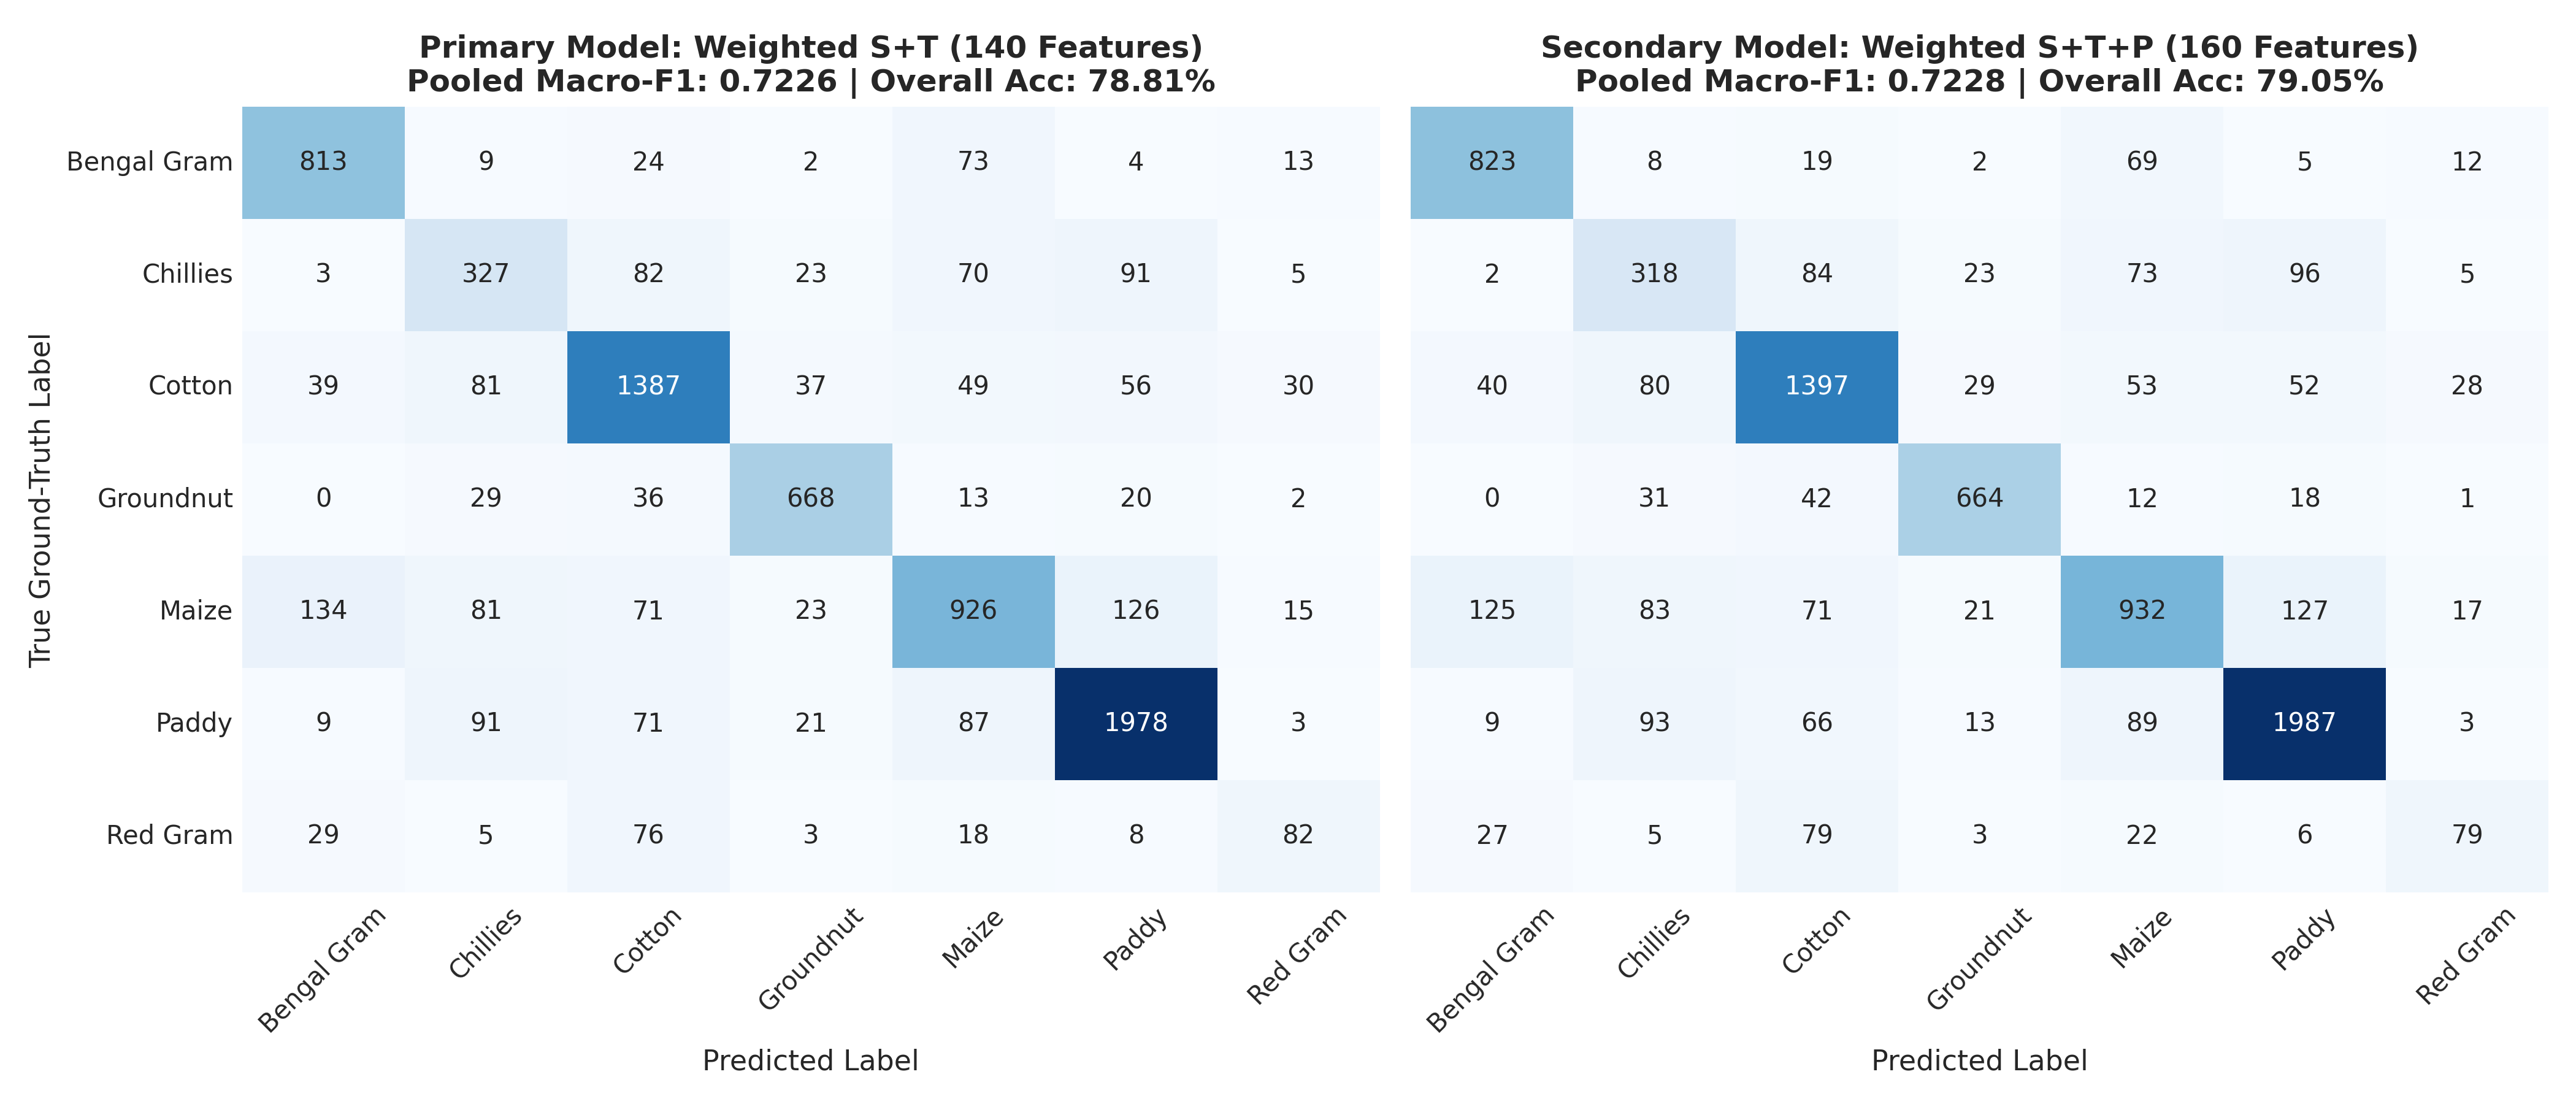
\includegraphics[width=0.75\textwidth]{outputs/reports/paper_materials/figures/fig1_confusion_matrices.png}
\caption{Normalized confusion matrices under 5-fold spatial cross-validation (left) and independent out-of-Mandal test evaluation (right).}
\label{fig:cm}
\end{figure}

\begin{figure}[t]
\centering
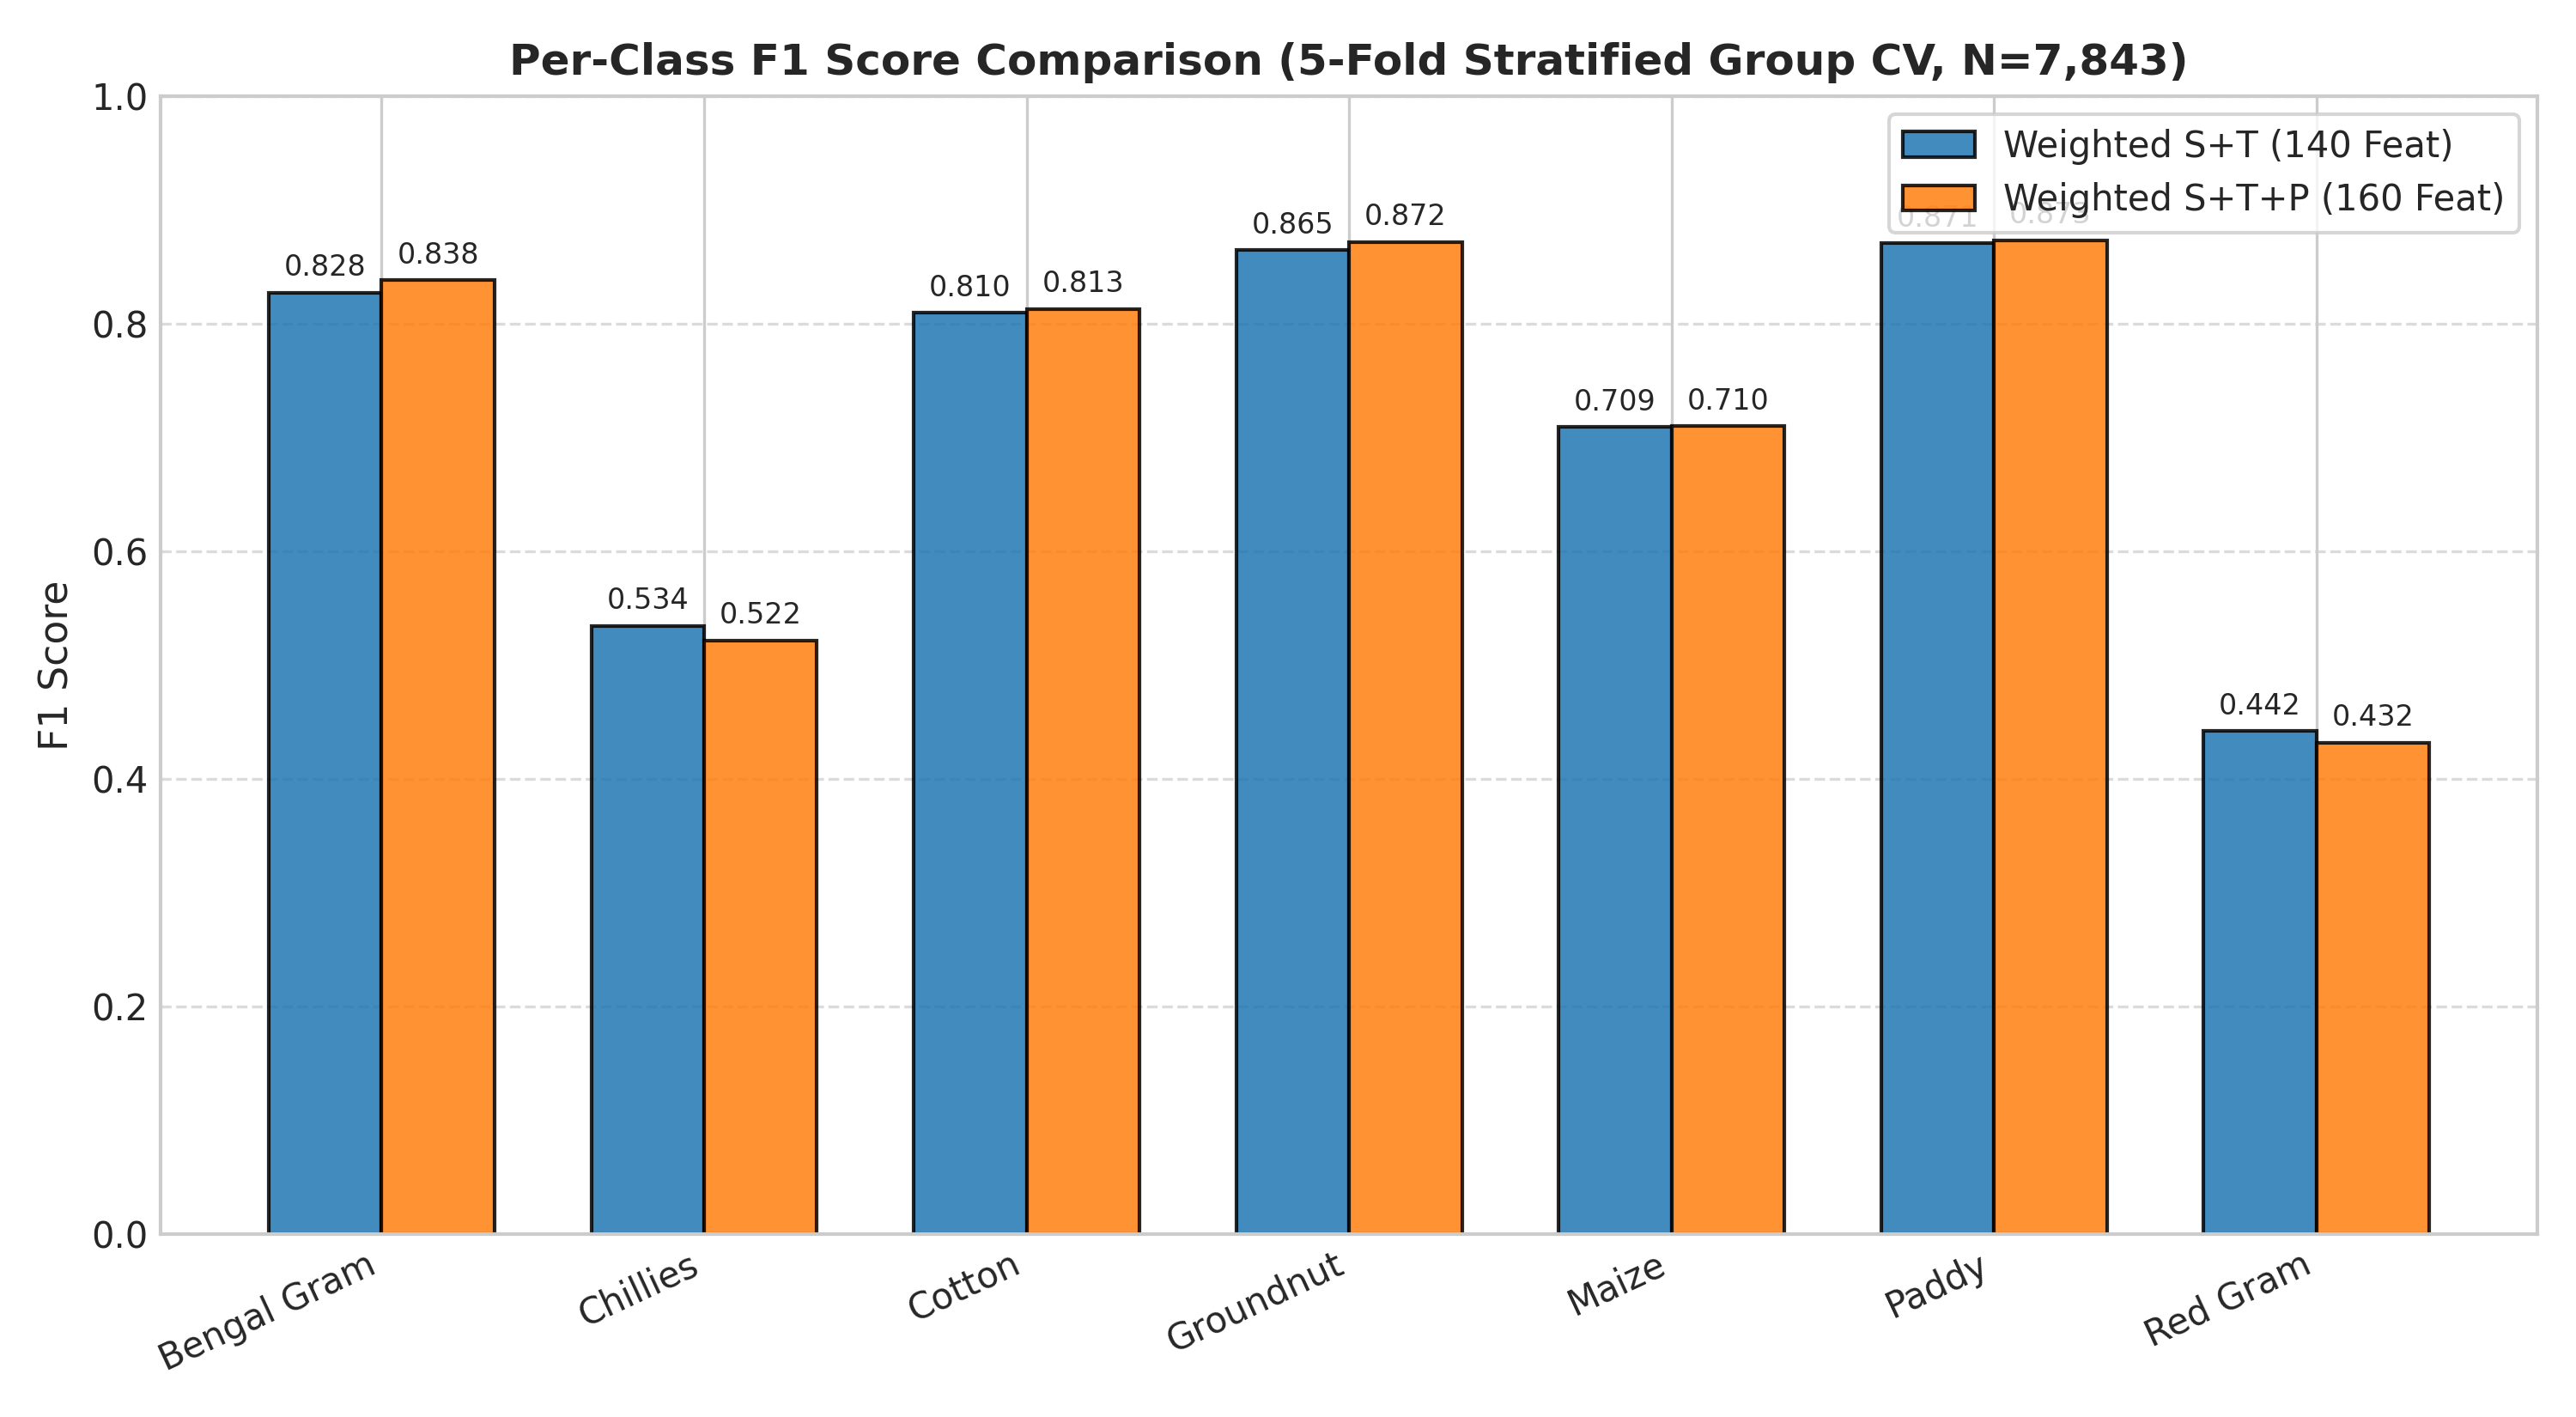
\includegraphics[width=0.7\textwidth]{outputs/reports/paper_materials/figures/fig2_class_wise_performance.png}
\caption{Class-wise precision, recall, and F1-score across seven crop types on the independent test set.}
\label{fig:classwise}
\end{figure}

\subsection{Interpretation of CV vs Test Scores}
Numerical test gains (0.7308 vs 0.7226) reflect class distribution shifts (Maize rose from 17.54\% to 27.86\% of parcels) and cloud-driven selection bias (Paddy lost 25.91\% of parcels vs 4.17\% for Bengal Gram), rather than superior geographic generalization.

\section{Limitations and Operational Constraints}
\begin{enumerate}
    \item \textbf{Cloud-Driven Attrition:} 16.67\% of test parcels were excluded due to persistent monsoon cloud obscuration.
    \item \textbf{Minority Class Fragility:} Red Gram test recall was 20.00\% ($N=35$ evaluated), with 60\% confused with Cotton due to overlapping sowing calendars and woody broadleaf canopies.
    \item \textbf{Single Cropping Year:} Evaluation is based on 2023 acquisitions; multi-year climate variability remains untested.
    \item \textbf{Geographic Scope:} Independent intra-state administrative holdout across 35 unseen Mandals within Telangana; ten broader districts overlap. Does not establish cross-state transfer or zero spatial autocorrelation.
    \item \textbf{Downstream Unimplemented Modules:} Disease diagnosis, ERA5 reanalysis, and FAO-56 irrigation scheduling are unvalidated future directions.
\end{enumerate}

\section{Conclusion}
This study established a reproducible benchmark for seven-class smallholder crop classification using multi-temporal Sentinel-2 imagery. A 140-feature Spectral-Temporal XGBoost model achieves 0.7226 spatial CV Macro-F1 and 0.7308 independent test Macro-F1 (81.55\% accuracy on 2,265 evaluated parcels). GLCM texture features provided no statistically supported benefit, and fold-internal weighting recovered minority pulse boundaries. Future work will integrate Sentinel-1 SAR to recover cloud-obscured parcels.

\subsubsection*{Acknowledgments}
\emph{[Acknowledgments and funding information omitted for double-blind peer review. Will be restored in camera-ready version upon acceptance.]}

\begin{thebibliography}{13}
\bibitem{defourny2019} Defourny, P., et al.: Near real-time agriculture monitoring at national scale at parcel resolution. Remote Sens. Environ. 221, 551--568 (2019)
\bibitem{jin2019} Jin, Z., et al.: Smallholder maize area and yield mapping at national scales with Google Earth Engine. Remote Sens. Environ. 228, 115--128 (2019)
\bibitem{griffiths2019} Griffiths, P., Nendel, C., Hostert, P.: Intra-annual reflectance composites from Sentinel-2 and Landsat for national-scale crop and land cover mapping. Remote Sens. Environ. 220, 135--151 (2019)
\bibitem{roberts2017} Roberts, D.R., et al.: Cross-validation strategies for data with temporal, spatial, hierarchical, or phylogenetic structure. Ecography 40(8), 913--929 (2017)
\bibitem{meyer2018} Meyer, H., et al.: Improving performance of spatio-temporal machine learning models using forward feature selection and target-oriented validation. Environ. Model. Softw. 101, 1--9 (2018)
\bibitem{vuolo2018} Vuolo, F., et al.: How much does multi-temporal Sentinel-2 data improve crop type classification? Int. J. Appl. Earth Obs. Geoinf. 72, 122--130 (2018)
\bibitem{lebourgeois2017} Lebourgeois, V., et al.: A combined Random Forest and OBIA classification scheme for mapping smallholder agriculture. Remote Sens. 9(3), 259 (2017)
\bibitem{inglada2015} Inglada, J., et al.: Assessment of an operational system for crop type map production using high temporal and spatial resolution satellite optical imagery. Remote Sens. 7(9), 12356--12379 (2015)
\bibitem{maxwell2018} Maxwell, A.E., Warner, T.A., Fang, F.: Implementation of machine-learning classification in remote sensing: An applied review. Int. J. Remote Sens. 39(9), 2784--2817 (2018)
\bibitem{chen2016} Chen, T., Guestrin, C.: XGBoost: A scalable tree boosting system. In: Proc. KDD '16, pp. 785--794. ACM (2016)
\bibitem{gumma2020} Gumma, M.K., et al.: Crop type identification and spatial mapping using Sentinel-2 satellite data with focus on field-level information. Geocarto Int. 37(13), 3824--3841 (2020)
\bibitem{gumma2022} Gumma, M.K., et al.: Multiple agricultural cropland products of South Asia developed using Landsat-8 30 m and MODIS 250 m data. GISci. Remote Sens. 59(1), 1048--1077 (2022)
\bibitem{haralick1973} Haralick, R.M., Shanmugam, K., Dinstein, I.: Textural features for image classification. IEEE Trans. Syst. Man Cybern. SMC-3(6), 610--621 (1973)
\end{thebibliography}

\end{document}
